%Master File:lectures.tex


\lesson{Graphical Models}
\vspace{-1cm}
\begin{center}
  \includegraphics[width=\linewidth]{GMplateLDA}
\end{center}
\keywords{Conditional Independence, Graphical models, LDA}
%%%%%%%%%%%%%%%%%%%%%%% Next Slide %%%%%%%%%%%%%%%%%%%%%%%
\renewcommand{\Outline}{%
\begin{slide}
\section[1]{Outline}

\begin{minipage}{10cm}\raggedright
  \begin{enumerate}\squeeze
    \outlineitem{Graphical Models}{graphicalmodel}
    \outlineitem{Cakes!}{cakes}
    \outlineitem{Latent Dirichlet Allocation}{lda}
  \end{enumerate}
\end{minipage}\hfill
\begin{minipage}{12cm}
  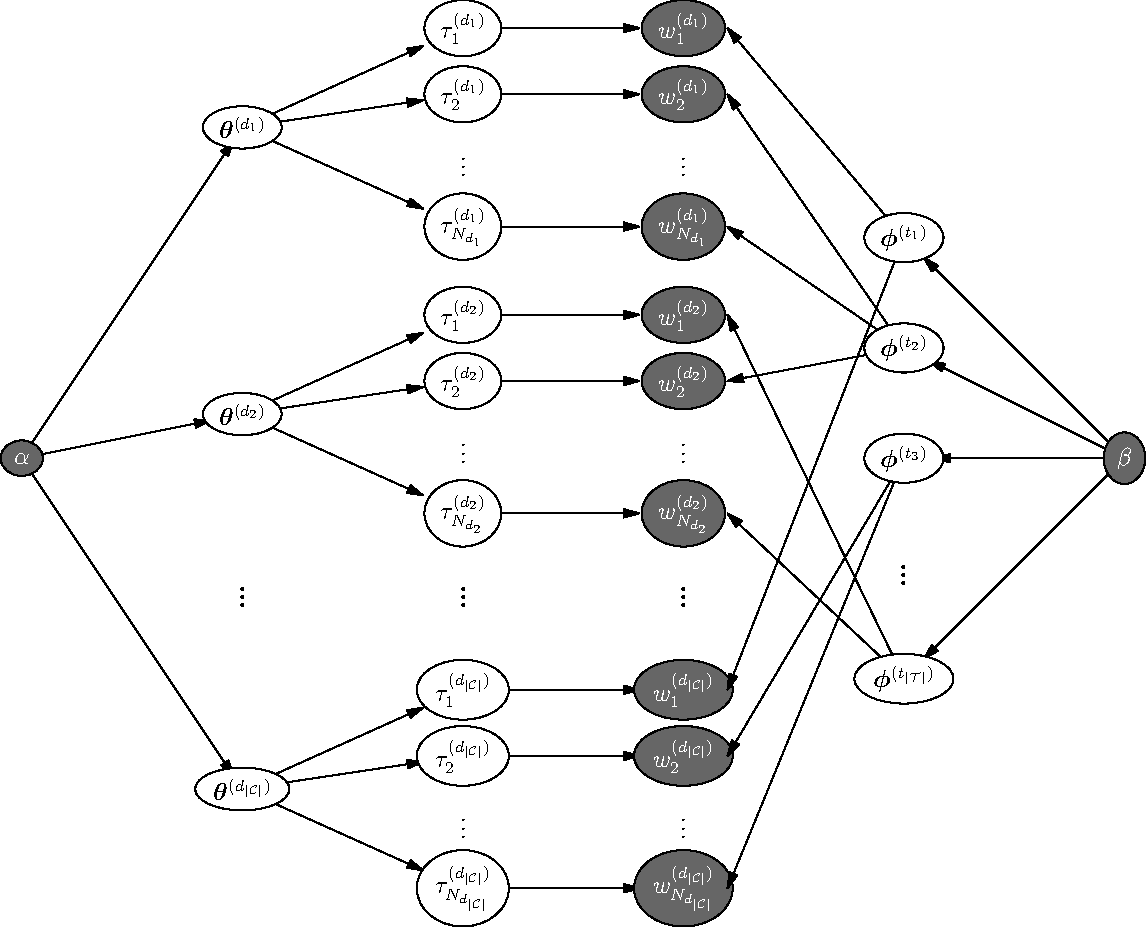
\includegraphics[width=12cm]{LDAGM}
\end{minipage}
\end{slide}
\addtocounter{outlineitem}{1}
}

\setcounter{outlineitem}{1}


%%%%%%%%%%%%%%%%%%%%%%% Next Slide %%%%%%%%%%%%%%%%%%%%%%%
\Outline % Graphical Models
\toptarget{firstoutline}
%%%%%%%%%%%%%%%%%%%%%%% Next Slide %%%%%%%%%%%%%%%%%%%%%%%

\begin{slide}
\section{Graphical Models}

\begin{PauseHighLight}
  \begin{itemize}
  \item If we want to build large probabilistic inference systems
    \begin{itemize}
    \item AI Doctor
    \item Fault diagnostic system for a computer
    \end{itemize}
    we can describe this by introducing random variables, but
    it is helpful to graphically represent causal connections\pause
  \item Graphical models allow us to do this\pause
  \item It allows us to build a joint probability from which we can
    compute everything we want\pause
  \end{itemize}
\end{PauseHighLight}

\end{slide}



%%%%%%%%%%%%%%%%%%%%%%% Next Slide %%%%%%%%%%%%%%%%%%%%%%%

\begin{slide}
\section{Dependencies Between Variables}

\begin{PauseHighLight}
  \begin{itemize}
  \item In building a probabilistic model we want to know which random
    variables depend on each other directly and which don't\pause
  \item Variables that don't will typically still be correlated\pause
  \item If two random variables $X$ and $Y$ are correlated then
    \begin{itemize}
    \item $X$ could affect $Y$
    \item $Y$ could affect $X$
    \item $X$ and $Y$ could not influence each other, but both be
      affected by another random variable $Z$\pause
    \end{itemize}
  \end{itemize}
\end{PauseHighLight}

\end{slide}

%%%%%%%%%%%%%%%%%%%%%%% Next Slide %%%%%%%%%%%%%%%%%%%%%%%

\begin{slide}
\section{Graphical Models}

\begin{PauseHighLight}
  \begin{itemize}
  \item \emph{Bayesian Belief Networks} are a type of graphical models
    where we use a directed graphs to show causal relationships
    between random variables\pause
  \item We could represent the three conditions described above by
    \begin{center}
      \includegraphics[width=0.4\linewidth]{simpleGraphicalModels}\pause
    \end{center}
  \item We can use these graphical representations to work out how to
    efficiently average over latent variables\pause
  \end{itemize}
\end{PauseHighLight}

\end{slide}

%%%%%%%%%%%%%%%%%%%%%%% Next Slide %%%%%%%%%%%%%%%%%%%%%%%

\begin{slide}
\section{Statistical Independence}

\begin{PauseHighLight}
  \begin{itemize}
  \item Two random variables are statistically independent if
    \begin{align*}
      \Prob{X,Y} = \Prob{X} \, \Prob{Y}\pause
    \end{align*}
  \item Equally this implies $\Prob{X|Y} = \Prob{X}$ and $\Prob{Y|X} =
    \Prob{Y}$\pause
  \item Statistically independent variables are uncorrelated\pause
  \item But statistical independence is often too powerful\pause
  \end{itemize}
\end{PauseHighLight}

\end{slide}

%%%%%%%%%%%%%%%%%%%%%%% Next Slide %%%%%%%%%%%%%%%%%%%%%%%

\begin{slide}
\section[-1]{Conditional Independence}

\begin{PauseHighLight}
  \begin{itemize}
  \item A weaker notion is conditional independence
    \begin{minipage}{0.68\linewidth}
      \begin{align*}
        \Prob{X,Y|Z} = \Prob{X|Z} \, \Prob{Y|Z}\pause
      \end{align*}
    \end{minipage}\hfil
    \begin{minipage}{0.18\linewidth}
      \begin{center}
        \includegraphics[width=\linewidth]{conditionalIndependence}
      \end{center}
    \end{minipage}
  \item Conditional independence implies that there is no direct
    causation\pause
  \item But it doesn't imply zero correlation\pause
  \item Conditional independence reduces computational complexity, e.g.
    {\small \begin{align*}
      \av{X\,Y} = \sum_{X,Y,Z} X\,Y \, \Prob{X, Y, Z} \pause
      = \sum_Z P(Z) \left(\sum_X X P(X|Z) \right)  \left(\sum_Y Y P(Y|Z)
      \right)\pause
    \end{align*}}
  \end{itemize}
\end{PauseHighLight}

\end{slide}


%%%%%%%%%%%%%%%%%%%%%%% Next Slide %%%%%%%%%%%%%%%%%%%%%%%
\Outline % Cakes
%%%%%%%%%%%%%%%%%%%%%%% Next Slide %%%%%%%%%%%%%%%%%%%%%%%

\begin{slide}
\section{Let Them Eat Cakes}

\begin{PauseHighLight}
  \begin{itemize}
  \item I will go through a very simple example involving cakes\pause
  \item It illustrates some simple principles\pause
  \item In the subsidiary notes I present a very simple program for
    computing all the probabilities\pause---I would encourage you to
    do this as it makes things much clearer\pauseb
  \end{itemize}
\end{PauseHighLight}

\end{slide}

%%%%%%%%%%%%%%%%%%%%%%% Next Slide %%%%%%%%%%%%%%%%%%%%%%%

\begin{slide}
\section[-2]{The Cake Scenario}

\begin{PauseHighLight}\squeeze
  \begin{itemize}
  \item Abi and Ben both bake cakes and bring them into the
    coffee room\pause
  \item Abi will bring in cakes 20\% of the time: \(\Prob{A=1} = 0.2\)\pause
  \item Ben will bring in cakes 10\% of the time: \(\Prob{B=1} = 0.1\)\pause
  \item 90\% of the time if either Abi or Ben have put cakes in the
    coffee room there is some left when I enter
    \(\Prob{C=1|A=1,B=0} = \Prob{C=1|A=0,B=1}=0.9\)\pause
  \item If they both make cake then there is always cake left  \(\Prob{C=1|A=1,B=1}=1\)\pause
  \item If neither Abi or Ben has made cake there is still a 5\%
    chance someone else has put cake in the coffee room \(\Prob{C=1|A=0,B=0}=0.05\)\pause
  \end{itemize}
\end{PauseHighLight}


\end{slide}

%%%%%%%%%%%%%%%%%%%%%%% Next Slide %%%%%%%%%%%%%%%%%%%%%%%

\begin{slide}
\section{Computing with Probabilities}

\begin{PauseHighLight}
  \begin{itemize}
  \item Other probabilities I can deduce,
    e.g. \(\Prob{C=0|A,B}=1-\Prob{C=1|A,B}\)\pause
  \item I can depict the causal relationship as
    \begin{center}
      
\includegraphics[width=0.3\textwidth]{figures/acb.pdf}\pause
    \end{center}
  \item The quantity that I really want is the joint probability
    \begin{align*}
      \Prob{A,B,C} &= \Prob{C,B|A}\,\Prob{A} \pause\\
                   &= \Prob{C|A,B}\,\Prob{B|A}\,\Prob{A}\pause
                    = \Prob{C|A,B}\,\Prob{B}\,\Prob{A}\pause
    \end{align*}
  \item Because \(\Prob{B|A}=\Prob{B}\)\pause
  \end{itemize}
\end{PauseHighLight}

\end{slide}

%%%%%%%%%%%%%%%%%%%%%%% Next Slide %%%%%%%%%%%%%%%%%%%%%%%

\begin{slide}
\section{Computing Expectations}

\begin{PauseHighLight}
  \begin{itemize}
  \item By using the joint probability and summing over all unknown
    quantities, we can compute expectations of anything we are
    interested in\pause
  \item These sums are often sped up using knowledge of conditional
    independence\pause
  \item To compute the probability of and event $\mathcal{E}$ we
    introduce an indicator function $\pred{\mathcal{E}}$ which is
    equal to 1 if the event happens and 0 otherwise
    $$ \Prob{\mathcal{E}} = \av{\pred{\mathcal{E}}} \pause $$
  \item If $E$ is a random variable equal to 1 if event $\mathcal{E}$
    happens and 0 otherwise then $E = \pred{\mathcal{E}}$\pause
  \end{itemize}
\end{PauseHighLight}

\end{slide}

%%%%%%%%%%%%%%%%%%%%%%% Next Slide %%%%%%%%%%%%%%%%%%%%%%%

\begin{slide}
\section{Are There Any Cakes Left?}

\begin{PauseHighLight}
  \begin{itemize}
  \item We can use our model to compute the probabilities of there
    being cakes in the coffee room
    \begin{align*}
      \Prob{C=1} &= \sum_{A,B,C\in\{0,1\}}
                   \pred{C=1}\, \Prob{A,B,C} \pause \\
      &= \sum_{A,B\in\{0,1\}}
       \Prob{C=1|A,B} \Prob{A}\,\Prob{B} = 0.29\pause
    \end{align*}
  \item The probability that Abi baked a cake is just 0.2 and for Ben
    its 0.1 (which is what we assume at the start)\pause
  \item The probability of them both baking on a particular day is 0.02\pause
  \end{itemize}
\end{PauseHighLight}

\end{slide}

%%%%%%%%%%%%%%%%%%%%%%% Next Slide %%%%%%%%%%%%%%%%%%%%%%%

\begin{slide}
\section{Making Observation}

\begin{PauseHighLight}
  \begin{itemize}
  \item Making observations changes probabilities\pause
  \item In graphical models observed random variables are shaded
    \begin{center}
      
\includegraphics[width=0.3\textwidth]{figures/acob.pdf}\pause
    \end{center}
  \item The probabilities conditioned on $C$ is given by
    $$ \Prob{A,B|C} =\frac{\Prob{A,B,C}}{\Prob{C}} \pause $$
    where
    $$ \Prob{C} = \sum_{A,B\in\{0,1\}} \Prob{A,B,C} \pause $$
  \end{itemize}
\end{PauseHighLight}

\end{slide}

%%%%%%%%%%%%%%%%%%%%%%% Next Slide %%%%%%%%%%%%%%%%%%%%%%%

\begin{slide}
\section{Who Made Those Cakes?}

\begin{PauseHighLight}
  \begin{itemize}
    \item If we observe there are cakes
    $$ \Prob{A,B|C=1} = \Prob{A,B,C=1}/\Prob{C=1} \pause $$
  \item A straightforward if tedious calculation shows
    \begin{align*}
      \Prob{A=1|C=1} &=0.628, &
      \Prob{B=1|C=1} &= 0.317 \\
      \Prob{A=1,B=1|C=1} &= 0.069 \pause
    \end{align*}
  \item Note \(\Prob{A=1,B=1|C=1} \neq \Prob{A=1|C=1} \,
    \Prob{B=1|C=1}\)\pause
  \item When we observe $C$ then $A$ and $B$ are no longer independent\pause
  \end{itemize}
\end{PauseHighLight}

\end{slide}

%%%%%%%%%%%%%%%%%%%%%%% Next Slide %%%%%%%%%%%%%%%%%%%%%%%

\begin{slide}
\section[-2]{Elaborate Cakes}

\begin{PauseHighLight}
  \begin{itemize}\squeeze
  \item We can elaborate on our cake model\pause
  \item We suppose that Dave likes cakes so if there is a cake in the
    coffee room there is a 80\% chance that I will see him eating a
    cake: \(\Prob{D=1|C=1}=0.8\)\pause
  \item Even if there are no cakes in the coffee room there is a 10\%
    chance that Dave has bought his own cake: \(\Prob{D=1|C=0}=0.1\)\pause
  \item Eli also likes cakes: there is a 60\% chance that I will see
    her eating cakes if there are cakes in the coffee room:
    \(\Prob{E=1|C=1}=0.6\)\pause
  \item But she never buys herself cakes \(\Prob{E=1|C=0}=0\)\pause
  \end{itemize}
\end{PauseHighLight}

\end{slide}

%%%%%%%%%%%%%%%%%%%%%%% Next Slide %%%%%%%%%%%%%%%%%%%%%%%

\begin{slide}
\section{Elaborate Graphical Model}
  
\begin{PauseHighLight}
  \begin{itemize}
  \item We can depict this situation as
    \begin{center}
      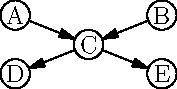
\includegraphics[width=0.3\textwidth]{figures/abcde_g.pdf}\pause
    \end{center}
  \item This allows us to break down the joint probability
    \begin{align*}
      \Prob{A,B,C,D,E} &= \Prob{C,D,E|A,B}\,\Prob{B}\,\Prob{A} \pause\\
                       &= \Prob{D|C}\,\Prob{E|C}\,
                         \Prob{C|A,B}\,\Prob{B}\,\Prob{A} \pause
    \end{align*}
  \item We use the conditional independence of $D$ and $E$ given $C$\pause
  \end{itemize}
\end{PauseHighLight}

\end{slide}

%%%%%%%%%%%%%%%%%%%%%%% Next Slide %%%%%%%%%%%%%%%%%%%%%%%

\begin{slide}
\section[-1]{Dependencies}

\begin{PauseHighLight}
  \begin{itemize}
  \item If we don't observe cakes then the probability of Dave and Eli
    eating cake are not independent
    \begin{align*}
      \Prob{D=1} &= 0.303, & \Prob{E=1} &= 0.174 \\
      \Prob{D=1,E=1} &= 0.1392\pause
    \end{align*}
    so \(\Prob{D,E}\neq\Prob{D}\,\Prob{E}\)\pauseb
  \item This changes if we know there are cakes in the coffee room
    \begin{align*}
      \Prob{D=1|C=1} &= 0.8 & \Prob{E=1|C=1} &= 0.6 \\
      \Prob{D=1,E=1|C=1} &= 0.48\pause
    \end{align*}
    so $\Prob{D=1,E=1|C=1}= \Prob{D=1|C=1}\, \Prob{E=1|C=1}$\pauseb
  \end{itemize}
\end{PauseHighLight}

\end{slide}


%%%%%%%%%%%%%%%%%%%%%%% Next Slide %%%%%%%%%%%%%%%%%%%%%%%

\begin{slide}
\section[-2]{Observations and Independence}

\pb
\begin{itemize}
\item Making observations changes the probabilities and in some case the
  dependencies of random variables
  on each other\pauseh
\end{itemize}
\begin{center}
  \multipdf[width=0.6\linewidth]{depend_abcde}\pause
\end{center}
\begin{itemize}
\item There are rules to deduce the conditional independence from a
  graphical model given which variables have been observed\pause---but
  these are details that you can look up if needed\pause
\end{itemize}
\end{slide}

%%%%%%%%%%%%%%%%%%%%%%% Next Slide %%%%%%%%%%%%%%%%%%%%%%%

\begin{slide}
\section{Graphical Model Frameworks}

\begin{PauseHighLight}
  \begin{itemize}
  \item There are sophisticated frameworks for computing probabilities
    in Bayesian Belief Networks efficiently\pause
  \item If our graph is a tree then we can evaluate probabilities
    efficiently\pause
  \item When there are loops (so that a random variable both influences
    and is influenced by another random variables) then exact
    evaluation of expectations requires exhaustive summing over
    variables\pause{} (which is often not tractable)\pauseb
  \item There are various message passing algorithms designed to
    obtain approximations of expectations\pause
  \end{itemize}
\end{PauseHighLight}

\end{slide}



%%%%%%%%%%%%%%%%%%%%%%% Next Slide %%%%%%%%%%%%%%%%%%%%%%%
\Outline % LDA
%%%%%%%%%%%%%%%%%%%%%%% Next Slide %%%%%%%%%%%%%%%%%%%%%%%

\begin{slide}
\section{Model for Documents}

\begin{PauseHighLight}
  \begin{itemize}
  \item We consider a model for the words in a set of documents (we
    ignore word order)\pause
  \item We consider a corpus $\mathcal{C} = \{d_i | i = 1,\, 2,\, \ldots
    |\mathcal{C}|\}$\pause
  \item With documents consisting of words
    \begin{align*}
      d = \left(w_1^{(d)},\, w_2^{(d)},\, \ldots,\, w_{N_d}^{(d)}\right)\pause
    \end{align*}
  \item We assume that there is a set of topics
    $\mathcal{T}=\{t_1,\,t_2,\,\ldots,\, t_{|\mathcal{T}|}\}$\pause
  \item We associate a probability, $\theta^{(d)}_t$, that a
    word in document $d$ relates to a topic $t$\pause
  \end{itemize}
\end{PauseHighLight}

\end{slide}

%%%%%%%%%%%%%%%%%%%%%%% Next Slide %%%%%%%%%%%%%%%%%%%%%%%

\begin{slide}
\section[-2]{Documents and Topic}
\begin{center}
  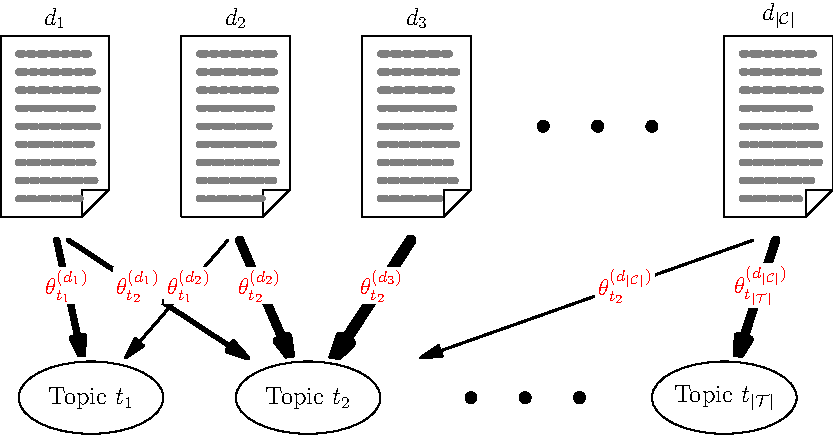
\includegraphics[width=\linewidth]{topicModelWtoT}\pause\\
  $\bm{\theta}^{(d)} = (\theta^{(d)}_t | t \in \mathcal{T}) \qquad
  \theta^{(d)}_t \geq 0 \qquad \sum\limits_{t=1}^{|\mathcal{T}|}
    \theta^{(d)}_t =1$
\end{center}
\end{slide}

%%%%%%%%%%%%%%%%%%%%%%% Next Slide %%%%%%%%%%%%%%%%%%%%%%%

\begin{slide}
\section{Words and Topic}

\begin{PauseHighLight}
  \begin{itemize}
  \item We associate a probability $\phi^{(t)}_w$ that a word, $w$, is
    related to a topic $t$\pause
    \begin{center}
      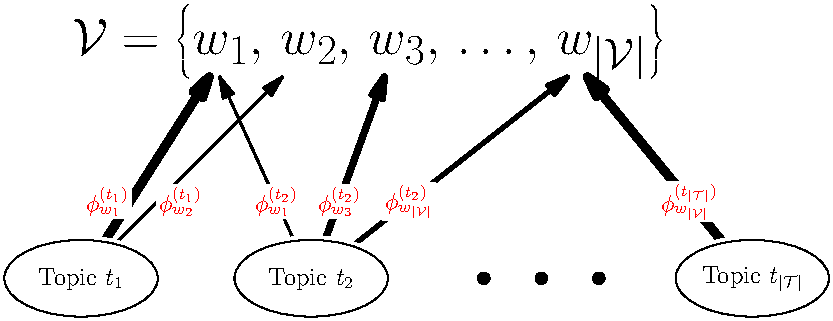
\includegraphics[width=0.7\linewidth]{topicModel}\\\ \\
      $\bm{\phi}^{(t)} = (\phi^{(t)}_w | w \in \mathcal{V})$\pause
    \end{center}
  \end{itemize}
\end{PauseHighLight}

\end{slide}

%%%%%%%%%%%%%%%%%%%%%%% Next Slide %%%%%%%%%%%%%%%%%%%%%%%

\begin{slide}
\section[-2]{Dirichlet Allocation}

\begin{minipage}{0.5\linewidth}
  \begin{PauseHighLight}
  \begin{itemize}
  \item Most documents are predominantly about a few topics and most
    topic have a small number of words associated to them\pause
  \item We can generate sparse vectors $\bm{\theta}^{(d)}$ and
    $\bm{\phi}^{(t)}$ from a Dirichlet distribution with small parameters
    $\bm{\alpha}$ 
    \begin{align*}
      \mathrm{Dir}(\bm{p}|\bm{\alpha}) = \Gamma\!\left(\sum_i
      \alpha_i\right) \prod_{i=1}^n
      \frac{p_i^{\alpha_i-1}}{\Gamma(\alpha_i)}
    \end{align*}
  \item $\sum\limits_{i} p_i=1$\pause
    \end{itemize}
\end{PauseHighLight}
\end{minipage}\hfil
\begin{minipage}{0.4\linewidth}
  \begin{center}
    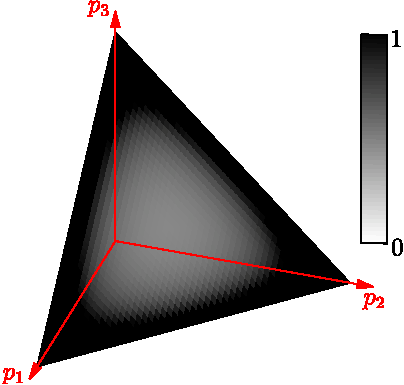
\includegraphics[width=0.95\linewidth]{dirichletSparse}\\
    $\bm{\theta}^{(d)} \sim \mathrm{Dir}(\alpha\,\bm{1})$\\
    $\bm{\phi}^{(t)}\sim \mathrm{Dir}(\beta\,\bm{1})$\pause
  \end{center}
\end{minipage}


\end{slide}

%%%%%%%%%%%%%%%%%%%%%%% Next Slide %%%%%%%%%%%%%%%%%%%%%%%

\begin{slide}
\section[-1]{Generating Document}

\begin{PauseHighLight}
  \begin{itemize}
  \item To generate a document we choose a topic for each word and a
    word for each topic\pause
    \begin{align*}
    \forall d\in\mathcal{C} \quad \bm{\theta}^{(d)}&\sim
    \mathrm{Dir}(\alpha\,\bm{1})\pause &&\\
    \forall t\in\mathcal{T} \quad \bm{\phi}^{(t)}&\sim
    \mathrm{Dir}(\beta\,\bm{1})\pause && \\
    \forall d\in\mathcal{C} \; \wedge\; \forall i\in\{1,\,2,\,\ldots, N_d\}
    \quad \tau^{(d)}_i &\sim \mathrm{Cat}(\bm{\theta}^{(d)}),\pause &
    w^{(d)}_i &\sim \mathrm{Cat}(\bm{\phi}^{(\tau^{(d)}_i)})
  \end{align*}
\item Where $\mathrm{Cat}(i|\bm{p}) = p_i$ is the categorical
  distribution (we choose one of a number of options)\pause
\item This model is known as \emph{Latent Dirichlet Allocation}\pause
  \end{itemize}
\end{PauseHighLight}

\end{slide}


%%%%%%%%%%%%%%%%%%%%%%% Next Slide %%%%%%%%%%%%%%%%%%%%%%%

\begin{slide}
\section[-2]{LDA Graphical Model (version 1)}

\pb\pause\pauselevel{=1}
\begin{center}
  \multipdf[width=0.8\linewidth]{LDAGM}\pause
\end{center}
\end{slide}

%%%%%%%%%%%%%%%%%%%%%%% Next Slide %%%%%%%%%%%%%%%%%%%%%%%

\begin{slide}
\section{Plate Diagrams}

\begin{PauseHighLight}
  \begin{itemize}
  \item Drawing every random variable is tedious (and not really
    possible)\pause
  \item A short-hand is to draw a box (plate) meaning repeat
    \begin{center}
      \includegraphics[width=0.5\linewidth]{GMplateSimple}\pause
    \end{center}
  \item That is we generate vectors $\bm{\theta}^{d}$ from a Dirchelet
    distribution $\Dist[Dir]{\bm{\theta}|\alpha \bm{1}}$ for all
    documents in corpus $\mathcal{C}$\pause
  \end{itemize}
\end{PauseHighLight}

\end{slide}


%%%%%%%%%%%%%%%%%%%%%%% Next Slide %%%%%%%%%%%%%%%%%%%%%%%

\begin{slide}
\section{LDA Graphical Model (version 2)}

\begin{center}
  \includegraphics[width=\linewidth]{GMplateLDA}
\end{center}
\begin{PauseHighLight}
  \begin{itemize}
  \item This is a lot more compact\pause
  \item Personally, I find it hard to read, but you get used to it\pause
  \end{itemize}
\end{PauseHighLight}

\end{slide}

%%%%%%%%%%%%%%%%%%%%%%% Next Slide %%%%%%%%%%%%%%%%%%%%%%%

\begin{slide}
\section[-2]{Probabilistic Model}

\begin{PauseHighLight}
  \begin{itemize}
\item The graphical Model is shorthand for the variables
 {\small \begin{align*}
    \bm{W} &= (\bm{w}^{(d)} | d\in\mathcal{C})\quad \text{with} \quad
    \bm{w}^{(d)}=(w_1^{(d)},\, w_2^{(d)},\, \ldots,\, w_{N_d}^{(d)}),
    \quad \text{and}\quad w_i^{(d)} \in \mathcal{V} \\
    \bm{T} &= (\tau^{(d)}_i | d\in\mathcal{C}\;\wedge\;
    i\in\{1,\,2,\,\ldots, N_d\})\quad \text{with} \quad \tau^{(d)}_i \in
    \mathcal{T} \\
    \bm{\Theta} &=(\bm{\theta}^{(d)} | d\in\mathcal{C})\quad \text{with}
    \quad \bm{\theta}^{(d)} = (\theta^{(d)}_t | t \in \mathcal{T})\in
    \Lambda^{|\mathcal{T}|} \\
    \bm{\Phi} &= (\bm{\phi}^{(t)} | t \in \mathcal{T}) \quad \text{with}
    \quad \bm{\phi}^{(t)} = (\phi^{(t)}_w | w \in \mathcal{V}) \in
    \Lambda^{|\mathcal{V}|}\pause
  \end{align*}}
\item Distributed according to
  {\small\begin{align*}
    \Prob{\bm{W},\bm{T},\bm{\Theta},\bm{\Phi}\big|\alpha,\beta} =
    & \left(\prod_{t\in\mathcal{T}} \Dist[Dir]{\bm{\phi}^{(t)}\big|\beta\bm{1}}\right)
    \\ & \Biggl(\prod_{d\in\mathcal{C}} \Dist[Dir]{\bm{\theta}^{(d)}\big|\alpha\bm{1}}
     \prod_{i=1}^{N_d} \Dist[Cat]{\tau_i^{(d)}\big| \bm{\theta}^{(d)}}
    \Dist[Cat]{w_i^{(d)} \big| \bm{\phi}^{(\tau_i^{(d)})}}\Biggr)\pause
  \end{align*}}

\end{itemize}
\end{PauseHighLight}

\end{slide}

%%%%%%%%%%%%%%%%%%%%%%% Next Slide %%%%%%%%%%%%%%%%%%%%%%%

\begin{slide}
\section{Finding Topics}

\begin{PauseHighLight}
  \begin{itemize}
  \item We are given the set of words $\bm{W}$ and don't really care
    about $\tau_i^d$ the topic associated with word $i$ in document
    $d$\pause
  \item But we are interested in the words associated with each topic
    $\bm{\phi}^{(t_i)}$\pause
  \item And the topics associated with each document
    $\bm{\theta}^{(d)}$\pause
  \item To compute them we need to sample the probability
    distribution\pause
  \item One way to do this is using Monte Carlo methods (see next
    lecture)\pause 
  \end{itemize}
\end{PauseHighLight}

\end{slide}


%%%%%%%%%%%%%%%%%%%%%%% Next Slide %%%%%%%%%%%%%%%%%%%%%%%

\begin{slide}
\section[-2]{Summary}

\begin{PauseHighLight}
  \begin{itemize}
  \item Building probabilistic models is an intricate process\pause
  \item Graphical models provide a representation showing the causal
    relationship between random variables\pause
  \item This allows us to break down the joint probability of all the
    variables into conditional probabilities\pause
  \item This is useful for building the model, but also can speed up
    evaluating expectations\pause
  \item Making observations changes the probabilities of random variables\pause
  \item It is possible to generate very rich models such as Latent
    Dirichlet Allocation (LDA)\pause
  \end{itemize}
\end{PauseHighLight}

\end{slide}

%%% Local Variables:
%%% TeX-master: "lectures"
%%% End:
